\documentclass[12pt,a4paper]{article}
\usepackage{fontspec}
\usepackage{xunicode}
\usepackage{polyglossia}
\setmainlanguage{french}
\usepackage{csquotes}
\usepackage{array}%tableaux améliorés (choix de la largeur de colonne)
\usepackage{graphicx}%insérer des images
\usepackage{lscape}%mettre en format paysage
\usepackage{tikz}%faire des graphiques
\usepackage{pgfplots}%graphiques à partir de données (courbes, histogrammes)
\usepackage{pgfplotstable}%importer les données depuis un fichier csv
\usepackage{longtable}%faire des tableaux sur plusieurs pages, insérer note dans des tableaux
\usepackage{url}
%\pgfplotsset{/pgf/number format/1000 sep=}%

\begin{document}
	
\section{Insérer des flottants}
\subsection{Images}

%1/Insérez ici l'image genealogie.jpg.
%2/Modifiez l'échelle de li'mage pour que ce soit satisfaisant
%3/ Transformez l'image en flottant. Indiquez où positionner le flottant.
%4/Ajoutez-lui une légende, ainsi que la source, qui se trouve ici: https://books.openedition.org/efr/2282
%5/ Faites-la tourner au format paysage
%6/ A la fin du document, insérez une liste des figures

\begin{landscape}
\begin{figure}[p]
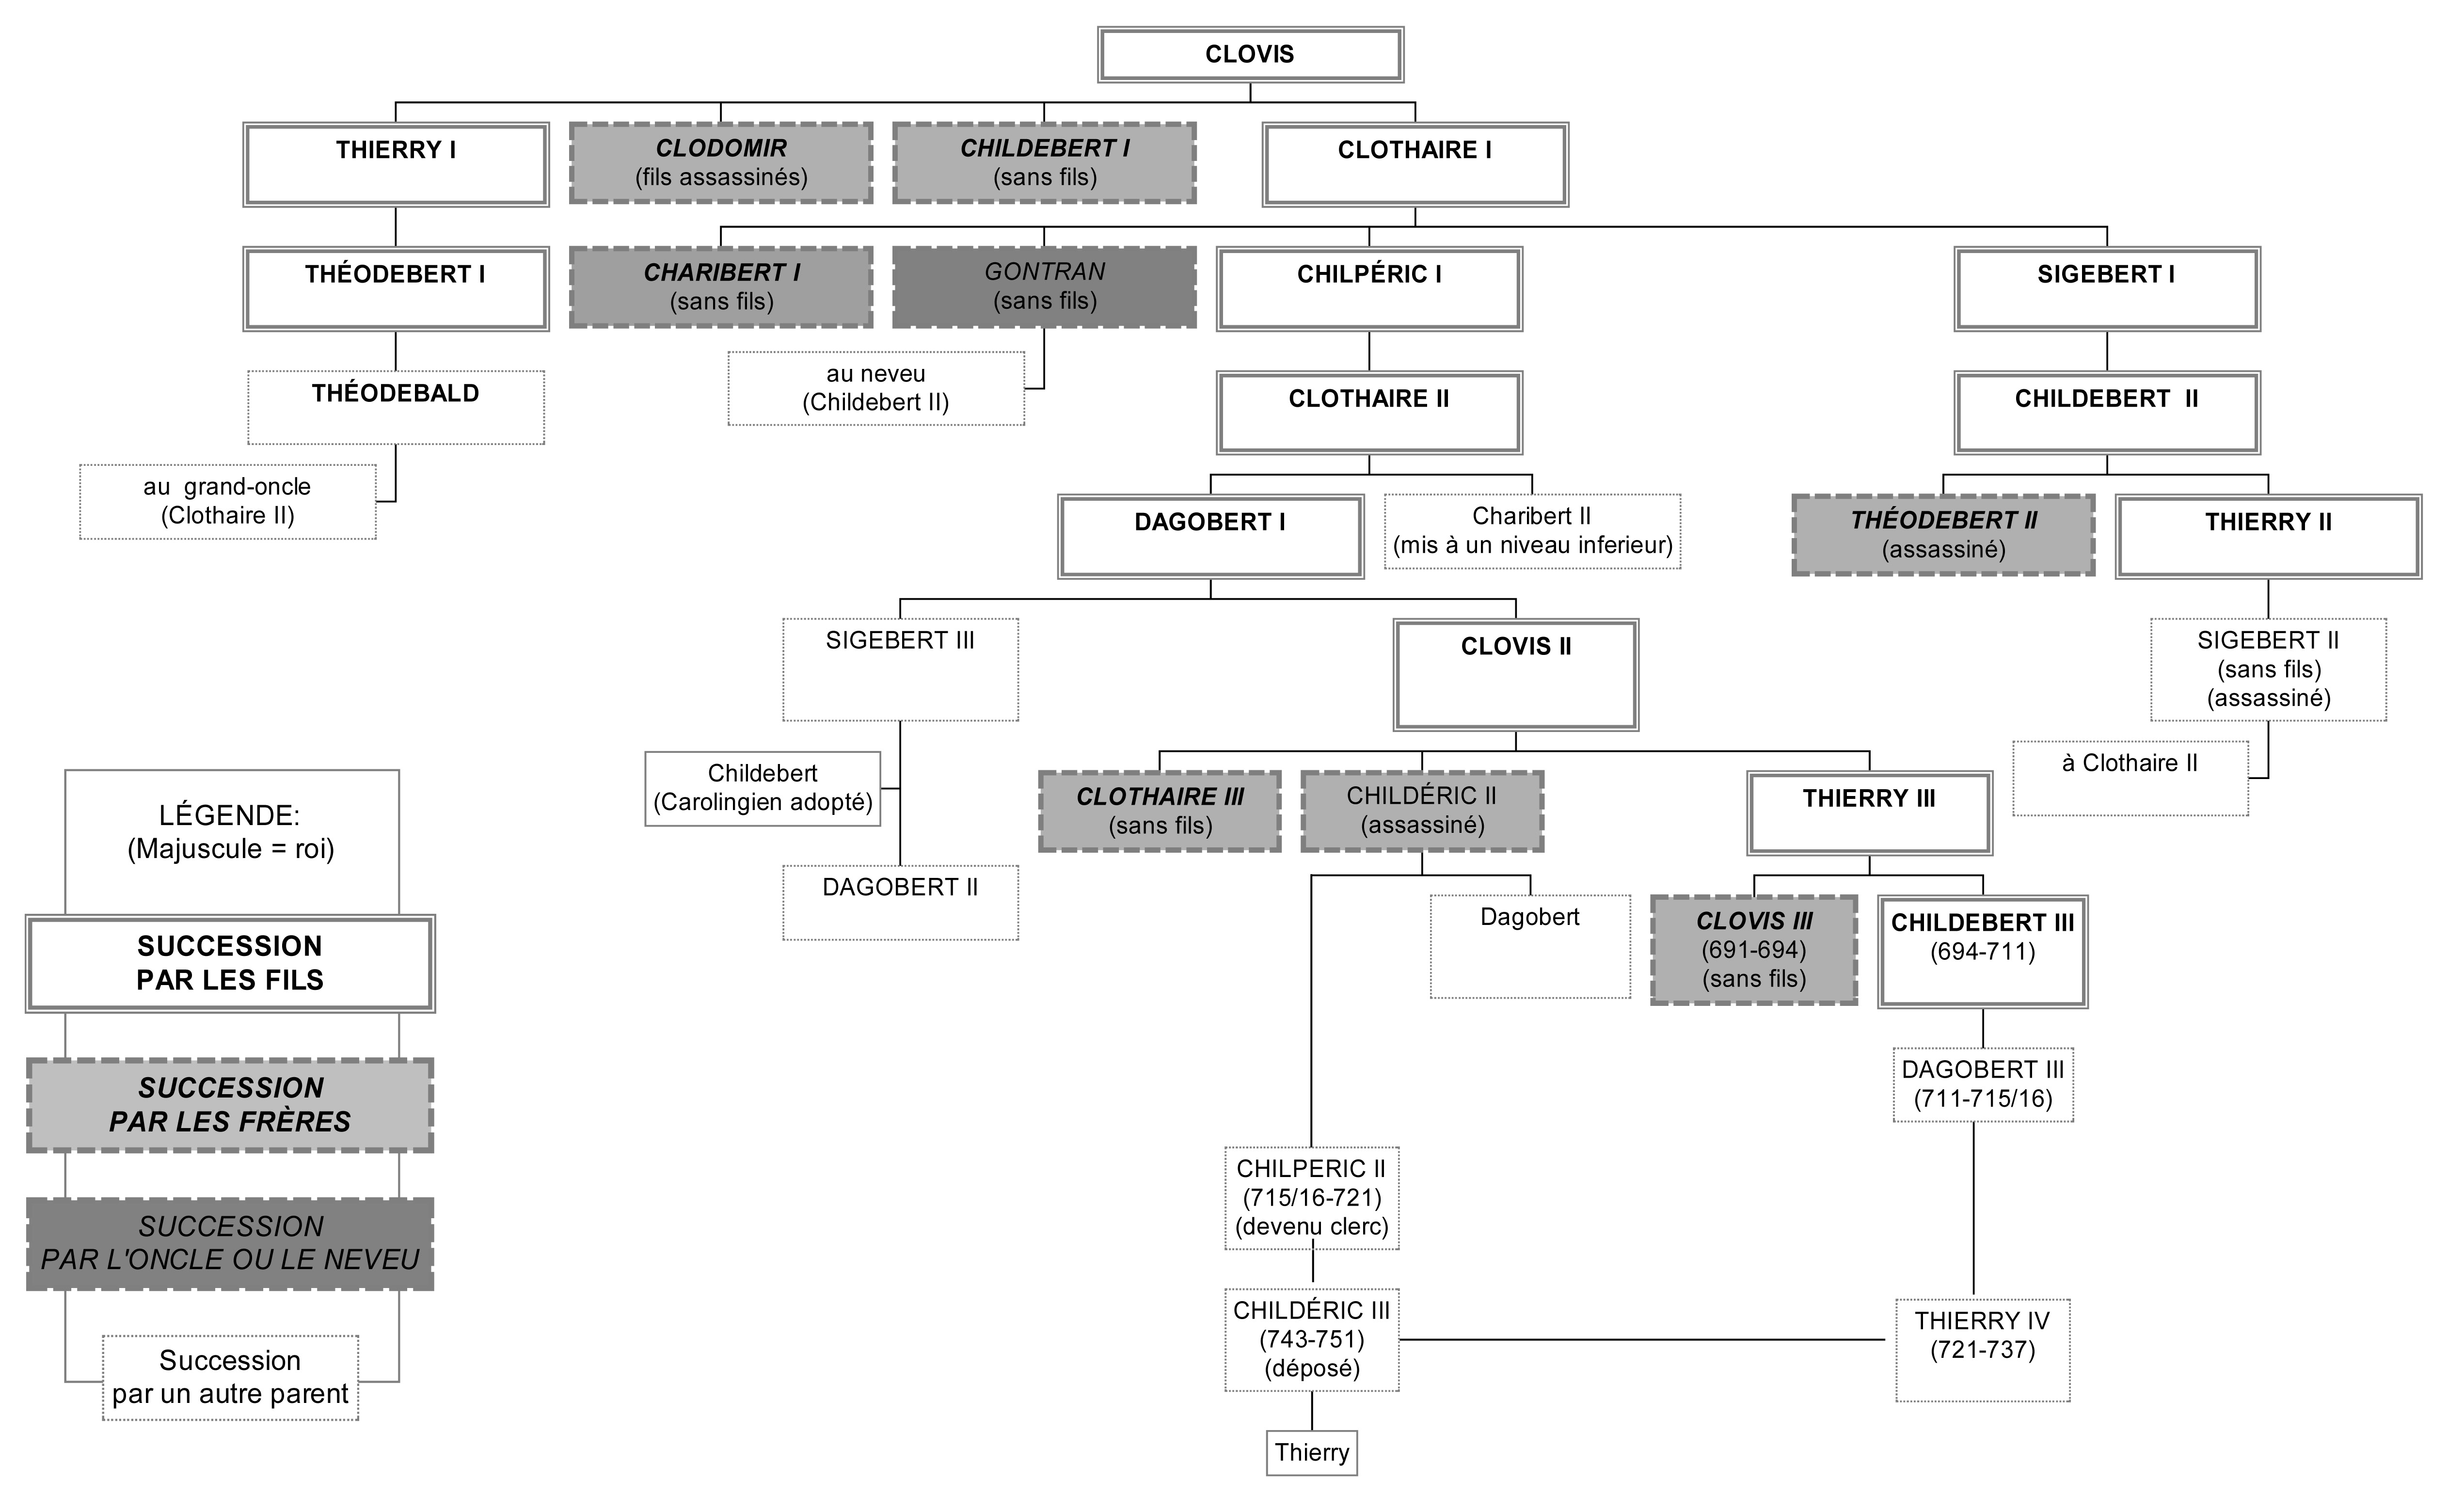
\includegraphics{genealogie.jpg}
\caption{légende.}
Source: \url{https://books.openedition.org/efr/2282}
\end{figure}
\end{landscape}

\subsection{Tableaux}

%1/en utilisant l'outil 'Assistant - Tableau ' de Texstudio: Insérez ici un tableau de trois colonnes et trois lignes; la première ligne des deux premières colonnes doit être fusionnée
%2/Observez comment le tableau est construit, puis rajoutez une ligne
%3/ Faites un autre tableau en choisissant pour les colonnes, dans l'option 'alignement', une des possibilités de 'largeur fixée'. Modifiez ensuite la largeur
%4/ Insérez une légende à vos tableau, et imprimez à la fin du document la liste des tableaux
\begin{table}
\begin{tabular}{|c|c|c|}
	\hline
	\multicolumn{2}{|c|}{Blop} & truc \\
	\hline
	A & B & C \\
	\hline
	D & E & F \\
	\hline
\end{tabular}
	\caption{un tableau}
\end{table}

\begin{table}
\begin{tabular}{|p{9cm}|m{9cm}|}
	\hline
	&  \\
	\hline
	&  \\
	\hline
\end{tabular}
	\caption{Un autre}
\end{table}

\subsection{Faire des graphiques avec tikz}

\subsubsection{Comprendre la syntaxe de tikz: l'exemple du \emph{stemma codicum}}

% Après avoir enlevé le signe %, ajoutez :
% a) un enfant à A, appelé D
% b) 1 enfant E à D
% Faites bien attention aux accolades. Indentez le code pour y voir plus clair
%mettez le tout dans un flottant, indiquez un paramètre de placement et ajoutez une légende
\begin{figure}[h]
\begin{tikzpicture}
\node {A}
	child {node {B}}
	child {node {C}}
	;

\end{tikzpicture}
\caption{arbre}
\end{figure}

\subsubsection{Tracer des diagrammes avec tikz  et pgfplot}

% Faire un schéma à partir du tableau 'travail_domestique_insee.csv' 
\begin{tikzpicture}
	\begin{axis}[xlabel=années, ylabel=temps de travail domestique]
		\addplot coordinates {(1986,2.07) (1999,2.13) (2010, 2.13)};
		\addplot coordinates {(1986,5.07) (1999,4.36) (2010, 4.01)};
		\legend{hommes,femmes}
	\end{axis}
\end{tikzpicture}

\section{Importer des données avec pgfplotstable pour produire tables et graphiques}

%Importez le tableau travail_domestique_insee.csv
\pgfplotstableread[col sep=comma]{travail_domestique_insee.csv}{\travail}
\pgfplotstabletypesetfile{\travail}

%importez ce tableau sous forme de diagramme
\begin{tikzpicture}[xscale=1.5]
	\begin{axis}[xtick=data]
		\addplot table[x=Date,y=Hommes]{\travail};
		\addplot table[x=Date,y=Femmes]{\travail};
	\end{axis}
\end{tikzpicture}

%Importez le tableau classement_prenoms_insee.csv sous forme d'histogramme en barres
\pgfplotstableread[col sep=comma]{classement_prenoms_insee.csv}{\prenoms}

\begin{tikzpicture}[xscale=1.5]
	\begin{axis}[ybar, xticklabels from table={\prenoms}{Prénom}, xtick=data, x tick label style={rotate=90}]%[ybar, xtick=data, xticklabels from table={\prenoms}{Prénom}, x tick label style={rotate=90}]
		\addplot table[x expr=\coordindex]{\prenoms};
	\end{axis}
\end{tikzpicture}

%\pgfplotstableset{
%	begin table=\begin{longtable},
%		end table=\caption{tableau 2}\end{longtable},
%	assign column name/.style={/pgfplots/table/column name={\textbf{#1}}},
%	string type,column type=l
%}
%Importez le tableau insee_categories_socio_professionnelles.ods. Attention, il faut auparavant le transformer en csv et le nettoyer.
\pgfplotstableread[col sep=tab]{insee_categories_socio_professionnelles.csv}{\table}


\pgfplotstabletypesetfile[string type,column type=l, begin table=\begin{longtable},	end table=\caption{tableau 2}\end{longtable},]{\table}


\section{Liste des figures et des tables}
%Insérer ici: une liste des figures et une liste des tables
\listoffigures
\listoftables






\end{document}